\documentclass[fleqn,10pt]{wlscirep}
\usepackage[utf8]{inputenc}
\usepackage[T1]{fontenc}
\usepackage{bm}
\usepackage{caption}
\usepackage{subcaption}
% \captionsetup[subfigure]{justification=justified,singlelinecheck=false}
\usepackage{tikz}
\usepackage{newtxmath} % MER: Prettier math
%\usepackage{natbib}
\usepackage{cleveref} % MER: Allows \Cref (but use Section X.Y not Subsection X.Y)
\usepackage{booktabs} % MER: Prettier tables

\usepackage{graphicx}
\usepackage{subcaption}
\usepackage{tikz}
\usepackage{float}
\usepackage{amsmath}
\usetikzlibrary{quotes}
\usetikzlibrary{arrows,decorations.pathmorphing,backgrounds,positioning,fit,petri}

\graphicspath{{figures/}}

\captionsetup[subfigure]{justification=justified,singlelinecheck=false}

\title{In-silico molecular transport in the human intracranial space}

\author[1,x]{Rami Masri}
\author[1,x]{Miroslav Kuchta}
\author[1,x]{Marius Causemann}
\author[1,*]{Marie E. Rognes}
\affil[1]{Department of Numerical Analysis and Scientific Computing, Simula Research Laboratory, Oslo, Norway}
\affil[x]{Author order to be discussed.}
\affil[*]{meg@simula.no}

\newcommand{\rami}[1]{\textcolor{blue}{#1}}
\newcommand{\mer}[1]{\textcolor{magenta}{#1}}
\newcommand{\discuss}[1]{\textcolor{red}{#1}}
\newcommand{\draft}[1]{\textcolor{gray}{#1}}
\newcommand{\brain}{\Omega_{\rm{brain}}} 
\newcommand{\sas}{\Omega_{\rm{SAS}}}
\newcommand{\pia}{\Gamma_{\rm{Pia}}}
\newcommand{\spinal}{\Gamma_{\rm{SC}}}
\newcommand{\skull}{\Gamma_{\rm{skull}}}
\newcommand{\gin}{g_{\rm{influx}}}
 % Hello darkness my old friend. I've come to talk with you again. 

%\affil[+]{these authors contributed equally to this work}

%\keywords{Keyword1, Keyword2, Keyword3}

\begin{abstract}
  TODOs:
  \begin{itemize}
  \item
    See notes in text
  \item
    Could Marius place meshes, especially the coarest one, somewhere
    accessible? Can be convenient to have actual mesh, not just code
    to generate it.
  \item
    Marie asks Hodneland about publishing the T1 data.
  \end{itemize}

\end{abstract}
\begin{document}

\flushbottom
\maketitle
% * <john.hammersley@gmail.com> 2015-02-09T12:07:31.197Z:
%
%  Click the title above to edit the author information and abstract
%
\thispagestyle{empty}



%%%%%%%%%%%%%%%%%%%%%%%%%%%%%%%%%%%%%%%%%%%%%%%%%%%%%%%%%%%%%%%%%%%%%%%%%%%%%%%%%%%%%
\section*{Introduction}

Molecular transport in perivascular spaces (PVSs) is established as a key pathway for human brain clearance and delivery. Previous studies indicate that molecules move rapidly in the subarachnoid space (SAS) and in PVSs surrounding pial arteries. Here, we aim to model and study this transport in a full pial perivascular and/or vascular network embedded in the SAS.  

\begin{itemize}
\item Vinje et al~\cite{vinje2021brain} and references therein illustrates the location and characteristics of human pial perivascular spaces.
\item Mestre et al~\cite{mestre2022periarteriolar} study the properties of pial perivascular spaces in detail in mice.
\item Mestre et al~\cite{mestre2018flow} measure and characterize pial perivascular transport and estimate flow magnitudes (in mice).
\item
  Weller and coauthors conducted pioneering studies of perivascular spaces, flow and transport~\cite{zhang1990interrelationships, zhang1992directional}. They identified thin sheaths of pial cells surrounding arteries and arterioles (but not veins or venules) on the brain surface and within the human brain itself~\cite{zhang1990interrelationships}. Further, they observed that tracers spread along perivascular (arterial, venous and capillar) spaces in (rat) grey matter, and in the subarachnoid space (to the cribriform plate and nasal lymphatics)..   
\item In a series of papers, Bakker and coauthors study perivascular anatomy and solute transport~\cite{bedussi2017paravascular, bedussi2018paravascular}. They find that the subarachnoid space, the cisterns, ventricles and penetrating periarteriolar spaces form a continuous cerebrospinal-fluid filled space surrounding and penetrating the rat brain\cite{bedussi2017paravascular}. Moreover, they demonstrate pulsatile and directional (antegrade) flow in perivascular (predominantly periarterial) spaces on the brain surface.
\item
  The architecture of pial and subarachnoid perivascular spaces in the rat brain was also studied by Thorne and colleagues~\cite{pizzo2018intrathecal, hannocks2018molecular}.
\item Bollman et al~\cite{bollmann2022imaging} image the human pial vasculature at high resolution (7T).
\item Hornkjøl et al~\cite{hornkjol2022csf} model CSF flow and solute transport in the human SAS and brain parenchyma. 
\item Mardal et al~\cite{mardal2022mathematical} give a succinct introduction to MRI-based computational brain modelling. 
\item
  Rey et al~\cite{rey2023perivascular} (from the group of Sartinoranont) model and study perivascular transport in rat brain networks.
\end{itemize}

%%%%%%%%%%%%%%%%%%%%%%%%%%%%%%%%%%%%%%%%%%%%%%%%%%%%%%%%%%%%%%%%%%%%%%%%%%%%%%%%%%%%%
\section*{Results}

\subsection*{High-fidelity in-silico predictions of intracranial solute transport and exchange}

\begin{itemize}
\item
  Present simulation results (outputs) from the baseline model (Model A, \Cref{tab:scenarios}). 
\item
  Highlight computational model availability, open source code -
\item
  Provides an interactive in-silico platform for studying intracranial solute transport -- distribute such that anyone can run (possibly try to recruit MinRK if advantageous).
\end{itemize}

\draft{\lipsum[1]}


\subsection*{Structural versus functional compartmentalization of perivascular spaces}

\begin{itemize}
\item
  Are perivascular spaces functionally or structurally
  compartmentalized? Human and rodent observations indicate that
  tracers concentrate in perivascular spaces surrounding the pial and
  subarachnoid vasculature. Must these spaces be structural
  i.e.~defined by semi-permeable structural membrane~\cite{zhang1990interrelationships, zhang1992directional, mestre2018flow, eide2024functional}, or can such
  compartmentalization be a result of regions of enhanced flow or
  mixing~\cite{bedussi2017paravascular, vinje2021brain}?
\item
  Compare Model A outputs with Models B--C (\Cref{tab:scenarios}).
\end{itemize}

\draft{\lipsum[1]}

\subsection*{The significance of low-resistance perivascular pathways}

\begin{itemize}
\item
  Perivascular flow and transport has been identified as a key
  mechanism and potential target for enhancing brain drug delivery and
  metabolic waste clearance -- what are the global (intracranial)
  effects of such intracranial highways? 
\item
  Compare Model A/B outputs with Models D--F (\Cref{tab:scenarios}).
\item
  Do solutes move from PVS to the SAS, or both along the PVS and along the SAS?
\end{itemize}

\draft{\lipsum[1]}

\begin{figure}
  \vspace{10em}
  \caption{Results: Perivascular flow}
  \label{fig:pvs}
\end{figure}

\subsection*{Clearance and the brain's waterscape}

\draft{\lipsum[1]}

\begin{itemize}
\item 
  Baseline model, but modelling metabolite clearance rather than solute
  influx (Model X). Consider several diffusion coefficients corresponding to
  gadubutrol, dextran, tau and amyloid-beta, otherwise identical flow
  set-ups. 
\item
  Compare clearance with a baseline model (with conservative flow)
  with a model with perivascular transport (Model Y) and full
  glymphatics (Model Z).
\end{itemize}

\subsection*{Intracranial solute influx and clearance during sleep}

\begin{itemize}
\item
  Sleep is known to affect a number of the transport characteristics including: increased extracellular volume fraction, altered vascular pulsatility and a-forteriori perivascular flow and mixing, reduced CSF production, reduced glymphatic transport (Model H).
\item
  Compare Model A/B with Model H, potentially also with a variation of Models X--Z (clearance, see below)
\end{itemize}

\draft{\lipsum[1]}

\subsection*{Influx and clearance in pathologies}

\begin{itemize}
\item
  A number of neurological and neurodegenerative disorders yield mechanical changes in the intracranial environment (increased arterial stiffness, cerebral arterial angiopathies, perivascular flow changes due to hypertension, altered CSF flow patterns, altered diffusion properties in cancer, BBB leakage) 
\item
  We select a few that we think are interesting/important and compare with baseline Model A/B for influx (drug delivery) or Models X--Z for clearance.
\end{itemize}

\draft{\lipsum[1]}



\iffalse
\newpage
\subsection*{Effect of interfaces (interface permeability)}

\begin{itemize}
    \item Model 0 (baseline): only diffusion, different diffusion coefficient in the parenchyma and SAS/PVS. No leak to vasculature (zero permeability). $\infty$ $\zeta_0$ at the PVS-SAS interface, $\zeta_1$ at the PVS-SAS interface. Koch et al could be a reference for PVS-parenchyma, maybe Tithof et al (2022, "A network model" ...) could give some ideas for parameters, also see Mestre et al, Nature comms, 2022. 
    \item 
    With altered interface permeabilities in the PVS (Model 1), and or in the parenchyma (Model 2) 
    \end{itemize}

\begin{figure}
    \caption{}
    \label{fig:1}
\end{figure}

\subsection*{Effect of convection}
\begin{itemize}
    \item 
    With convective flow in the PVS (zero flow in the parenchyma for now)
    \begin{itemize}
        \item 
        Model 3: PVS flow equal to 18.7 $\mu$m/s
        \item 
        Model 4: Better PVS flow (distributed, according to conservation of mass, assumptions on PVS area)
    \end{itemize}    
    \item 
    With convective flow in the ECS (out of scope here, for follow-up work?)
\end{itemize}

\begin{figure}
    \centering
    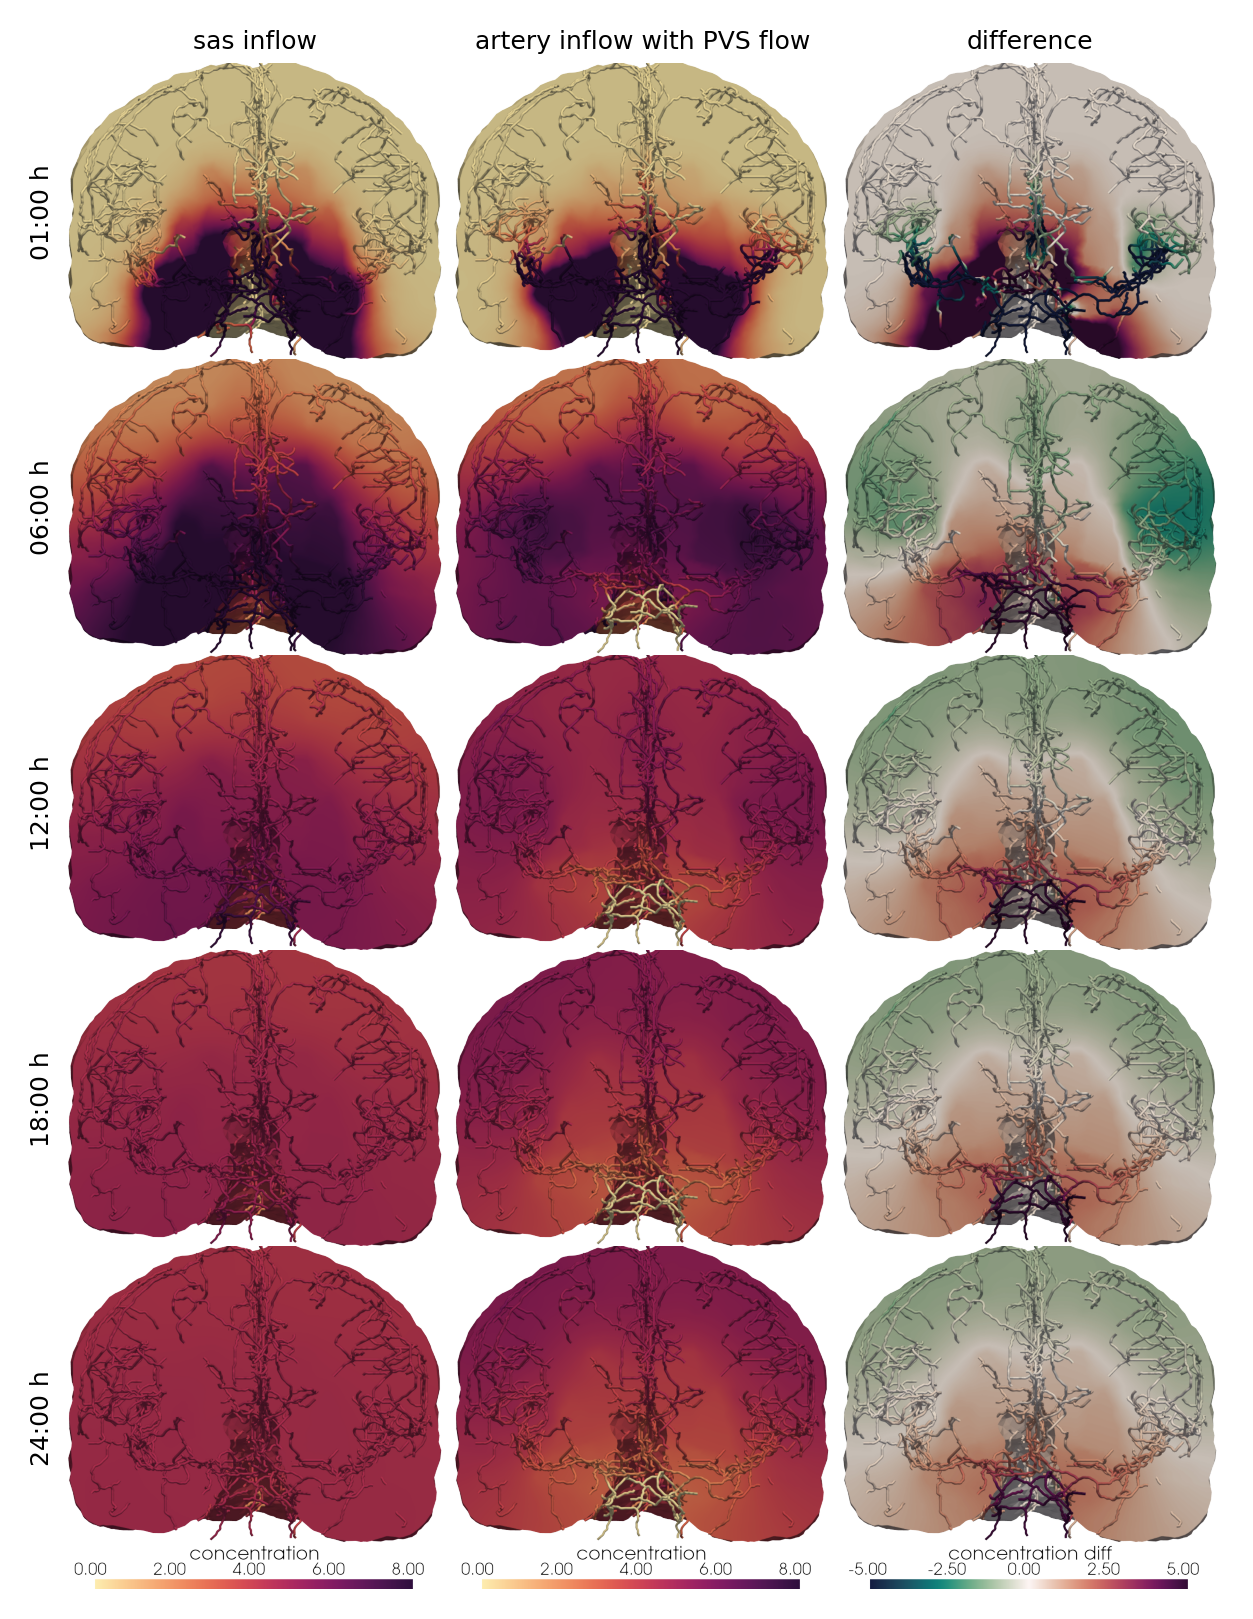
\includegraphics[width = 0.9 \textwidth]{modelB_modelC_overview.png}
    \caption{Tracer concentrations for a purely diffusive model with tracer inflow via the CSF-filled space (left) and a convective model with Tracer inflow via the arterial PVS (middle) and their difference (right) at 1, 6, 12, 18 and 24 hours after injection.}
    \label{fig:2}
\end{figure}
\subsection*{Effect of BBB}

Leakage to the blood, some sink/non-zero permeability for the PVS-blood (BBB) interface (Model N).

\begin{figure}
    \caption{}
    \label{fig:3}
\end{figure}

\subsection*{Effect of pia}
  
Effect of pia permeability (Model N-1)    

\begin{figure}
    \caption{}
    \label{fig:4}
\end{figure}

\begin{figure}
     \centering
     \begin{subfigure}[b]{0.33\textwidth}
         \centering
         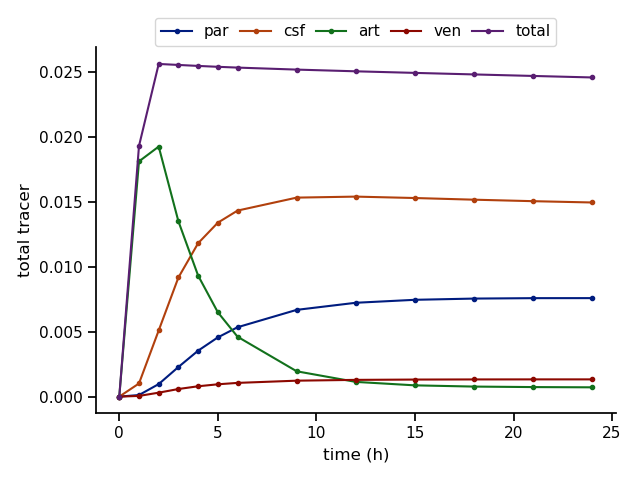
\includegraphics[width=\textwidth]{modelA_total_conc.png}
         \caption{arterial inflow, pure diffusion}
         \label{fig:y equals x}
     \end{subfigure}
     \hfill
     \begin{subfigure}[b]{0.33\textwidth}
         \centering
         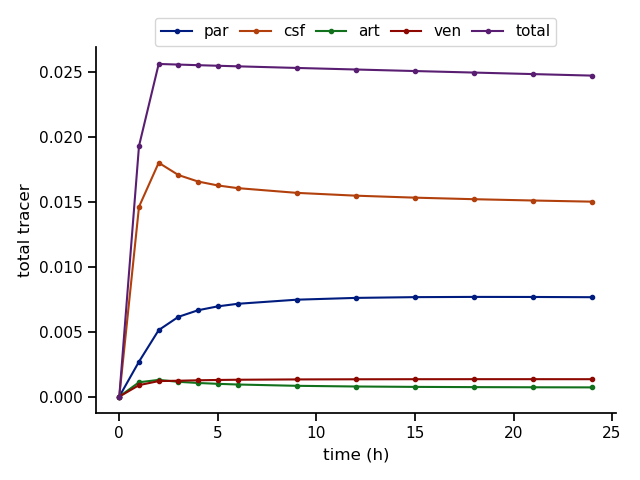
\includegraphics[width=\textwidth]{modelB_total_conc.png}
         \caption{SAS inflow, pure diffusion}
         \label{fig:three sin x}
     \end{subfigure}
     \hfill
     \begin{subfigure}[b]{0.33\textwidth}
         \centering
         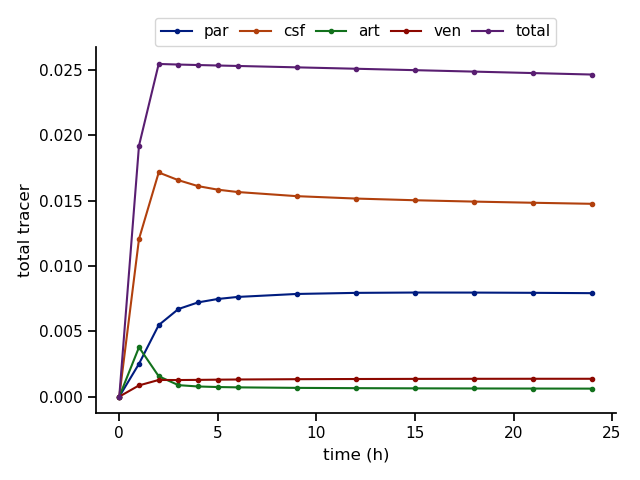
\includegraphics[width=\textwidth]{modelC_total_conc.png}
         \caption{arterial inflow, diffusion + PVS convection}
         \label{fig:five over x}
     \end{subfigure}
        \caption{Total tracer amount in parenchyma, CSF, arterial PVS and venous PVS}
        \label{fig:three graphs}
\end{figure}

\fi

\newpage
%%%%%%%%%%%%%%%%%%%%%%%%%%%%%%%%%%%%%%%%%%%%%%%%%%%%%%%%%%%%%%%%%%%%%%%%%%%%%%%%%%%%%
\section*{Methods}

%\mer{MER: I recommend writing each (sub)section of Methods as a nearly stand-alone paragraph. Let's see if we can avoid subsubsections/paragraphs. If you need to add more detail than you think is appropriate, put it in a Supplementary Methods section in the Appendix.} 

\subsection*{Brain parenchyma, SAS, and interface geometries}

\mer{MER: Suggestion @Marius: Would you have a go a refining this section? Keep it brief. Mention number of cells and max/min mesh size. I like including references to tools used as you have done. Refer to \Cref{fig:concept}. Include units when describing the geometry. Clearly illustrate the boundaries in the Figure, and refer to these in the text. Description should be such that it is easily to intuitively understand, but perhaps not reproduce immediately (that is why we will also share the code).}  


Hodneland et al~\cite{hodneland2019new} developed a method to image
the brains' microvasculature based on time-of-flight (ToF) and
quantitative susceptibility mapping (QSM) to identify arterial and
venous networks.  We derive a detailed tetrahedral mesh of the
parenchyma and the surrounding CSF-filled spaces alongside a network
representation of the vasculature from the anatomical data provided
therein. We merge the white and grey matter masks provided by
\cite{hodneland2019new} to extract the pial surface.
 


As no data on the CSF-filled spaces is available, we smooth and extend
the pial surface by about 5\,mm to obtain an approximation of the SAS
and include the inner fluid-filled cavities such as the ventricular
system.  Finally, we generate a tetrahedral mesh of both compartments
using the fTetWild meshing algorithm \cite{hu2020fast}.

The computational domain $\Omega$ is defined by the union of the SAS $\Omega_{\rm sas}$ and brain parenchyma $\Omega_{\rm brain}$. The thin pia membrane encloses the brain, and thus the pial surface (of the brain) defines the SAS-brain interface $\Gamma_{\rm pia}$.


Surface representations of the outer SAS boundary, pial membrane, and delimiters of other CSF-filled spaces such as the lateral ventricles, third and fourth ventricle, and aqueduct are extracted from MR-images of human subject(s), see e.g. the pipeline described by Hornkjøl et al.~\cite{hornkjol2022csf}. From these surface representations, we create volumetric meshes of the SAS and brain using SVMTK~\cite{mardal2022mathematical}. 

We mark the different regions of the boundary of $\Omega$, with
$\Gamma_{\mathrm{skull}}$ facing the dura and skull and
$\Gamma_{\mathrm{spine}}$ representing the lower interface towards the
spinal compartment (\Cref{fig:concept}).  We also the interface between the $\Omega_{\rm{brain}} $ and $\Omega_{\rm{SAS}}$ by  $\Gamma_{\rm{Pia}}$. The boundary of the spinal canal is denoted by $\Gamma
_{\rm{SC}}$ which is given by $\Gamma_{\rm {SC}} \backslash \Gamma_{{brain}}$. \mer{MER: I put this here, keep
  it here. How about the ventricles?}

\subsection*{Vascular and perivascular domains and networks}

\mer{Is this up-to-date? @Rami checks sanity and numbers of paragraph.}

We skeletonize the binary masks of the arteries and veins of the
Hodneland~\cite{hodneland2019new} data set using
Kiminaro~\cite{william_silversmith_2021_5539913}, to obtain the
centerline $\Lambda^i$ and radius $R_1^i$ of each detected vessel $i$,
and the vessel connections. The resulting vascular networks are
further smoothened using a spline interpolation technique, and
represented as graphs with nodes connected by edges. The arterial
network contains 11862 nodes (and 11861 edges), while the venous
network contains 21883 nodes (and 21882 edges); with no cycles in
either network. Nodes connected to only one edge (i.e.~with graph
degree 1) are labelled terminal nodes. For the arterial network, we
identify 3 of the terminal nodes, representing \mer{the two internal
  carotid arteries and the basilar artery}, as root nodes
(\Cref{fig:concept}) and label the other terminal nodes as leaf
nodes. \mer{Range of lengths of the networks paths.} We denote the
domain defined by the connected centerlines by $\Lambda$. The vascular
domain is then represented as the union of cylindrical vessels of
radius $R_1^i$ surrounding the centerlines $\Lambda^i$. Moreover, we
consider the surrounding perivascular spaces as the union of annular
cylinders of inner radius $R_1^i$ and outer radius $R_2^i = \beta R_1^i$ of width $R_2^i - R_1^i = (\beta - 1) R_1^i$. Both the
vasculature and perivasculature are thus defined relative to a common
network of vessel segments.

\begin{figure}
  \caption{@Marius: Starts adding parts of this. \mer{MER: Concept figure illustrating the compartments and story line. (A) Concept sketch of the SAS, PVS and the brain; (B) Visualization of geometry domains (brain, sas and vasculature; think about colors and associations; please don't make blood blue and water red e.g.) ; (C) Zoom-in/detail on vasculature, which are which arteries (ACA, MCA, PCA, CoW)  and veins (XXX); (D) Zoom-in 2 on vascular position versus SAS and brain; (E) Zoom-in 3 on where PVS ends; (F) Illustration of boundaries? (G) Concept illustration of the mathematical model (diffusion, convection, exchange, boundaries).}}
\label{fig:concept}
\end{figure}

\subsection*{Multi-dimensional intracranial transport equations}

\mer{@Rami revisits. Is the interface jump condition the right one? Rami will draft, Marius will check versus code. In text, refer to Table for parameters.}

We model diffusion, convection and exchange of a solute in PVSs, in the surrounding SAS and in the brain parenchyma (Fig.~\ref{fig:concept}) via a comprehensive multi-dimensional transport model~\cite{masri2023modelling} over a timescale of minutes to hours. More specifically, we solve for a solute concentration $c$ (defined locally in each subdomain $\Omega_{\rm{brain}}$ and $\Omega_{\rm{SAS}}$ in the 3D SAS and brain~\cite{sykova2008diffusion} $\Omega$, and an averaged solute concentration $\hat c$ in a 1D network of centerlines $\Lambda$ representing the PVS, such that the following equations hold
\begin{subequations}
\begin{alignat}{2}
  \partial_t (\phi c) - \nabla \cdot (D \nabla (\phi c) ) + \nabla \cdot (\bm u c ) + \xi (\overline{c} - \hat c ) \delta_\Gamma & = f && \quad \quad \mathrm{in} \quad \Omega_{\rm{SAS}} \cup \Omega_{\rm{brain}}, \label{eq:multi_transport_3d} \\ 
  \partial_t (A \phi \hat c) - \partial_s(\hat D A \partial_s (\phi \hat c)) +\partial_s(A \hat u \hat c )  +  \xi P (\hat c - \overline{c})  &= A \hat f && \quad \quad \mathrm{in} \quad  \Lambda . \label{eq:multi_transport_1d}
 \end{alignat}
\end{subequations}
Here $\phi$ is the fluid volume fraction (or porosity) of the brain (where $\phi \ll 1$), of the SAS (where $\phi = 1$) and of the PVS (where $0 \ll \phi \leq 1$); $D$ is the effective diffusion coefficient of the relevant solute in the respective media~\cite{sykova2008diffusion} which takes different values over the SAS, PVS, and tissue; $\bm u$ and $\hat u$ are convective velocity fields in $\Omega$ and $\Lambda$, respectively; $\xi$ is a transfer coefficient across the PVS-SAS interface; $P$ and $A$ are the perimeter and area of the PVS which can vary along the centerline network, respectively; and $f$ and $\hat{f}$ represents given sources of solute in $\Omega$ and $\Lambda$, respectively.   The velocity field $\bm u$ takes different values over $\Omega_{\rm {SAS}} $ and $\Omega_{\rm{brain}}$, see for example \Cref{tab:scenarios} and \Cref{sec:csf_fluid_vel} and \Cref{sec:csf_brain}. Similarly $\hat u$ takes different values on each $\Lambda_i$, see for example \Cref{sec:csf_pvs}.

The (Dirac delta) term $\delta_\Gamma$ is a source term concentrated on the outer boundary of the PVS that models the solute exchange between the PVSs and their surroundings. Finally, the notation $\overline{c}$ denotes the lateral  average of the concentration over the outer perivascular boundary. Both $\Omega$ and $\Lambda$ are here fixed in time. We remark that this version of the model assumes that there is no interaction between the inner perivascular boundary and the blood vessel. 

%\noindent \mer{MER: @Rami: I've added the $\phi$'s in this subsection. Please review and add convective terms in $\Omega$ and $\Lambda$.} \rami{done, maybe I include a more precise variational formulation in the appendix ? }
\subsection*{Initial conditions}

We set the initial concentrations $c_0, \hat{c}_0$ in the three-dimensional domain $\Omega$ and network $\Lambda$ to be zero for all influx scenarios (Models A--\draft{X-1}). For modelling clearance (Model \draft{X}), we set $c_0 = 1, \hat{c}_0 = 0$.

\subsection*{Boundary conditions: extracranial efflux and perivascular parenchymal influx}

On $\Gamma_{\mathrm{skull}}$, the interface towards the dura and skull , we consider a constant uptake (or efflux) rate, represented by the boundary condition $- D \nabla c \cdot \bm{n} + \bm u \cdot \bm n c  = \beta c $ (\Cref{fig:concept}) where $\beta$ represents a molecular outflow resistance. Here, we take $\beta = 10^{-4} \,\, \mathrm{mm}^2/\mathrm{s}$\cite{hornkjol2022csf}.
\mer{Marius says that this $\beta$ makes the solute accumulate. Maybe we want to modify this parameter.}

On $\Gamma_{\mathrm{spine}}$, the interface towards the spinal compartment , we prescribe a time-dependent solute influx rate by the condition $D \nabla c \cdot \bm{n}  -  \bm u \cdot \bm n  c = g_{\mathrm{influx}}(t) \geq 0$ representing the distribution of solute injected in the spinal compartment. Here, we set $g_\mathrm{influx}(t) = \max(0, \kappa (T_0 - t))$ where $\kappa  = $ and $T_0 = $. \mer{@Marius: modify this above paragraph to reflect the current approach.}
% \rami{marius, double check in the code they are different than \cite{hornkjol2022csf}}. 


\mer{@Marius: Could you edit the paragraph below to reflect the simplified set-up (which we can because of the improved geometry.)}
On the associated perivascular network inlet nodes $\partial \Lambda_{\mathrm{in}}$ (\Cref{fig:concept}), we prescribe a homogenous Neumann condition $\hat D A \partial_s (\phi \hat c) - A \hat u \hat c  = 0 $. For the vessels that 
lie in a sphere of radius of $0.04$ located at the base of the third ventricle, we set the permeability  $\xi_{\rm{PVS,CSF-BC}}= 100\xi_{\rm{PVS,CSF}}$ . For the "leaf" nodes of the perivascular network (representing the end of the surface perivascular network and start of perivascular spaces within the parenchyma), we also sel homogenous Neumann boundary conditions $ D A \partial_s (\phi \hat c) - A \hat u \hat c  = 0 $ . % g_{\mathrm{pvs-par}}$.  
% \rami{I don't think we can have anything different than $g_{\mathrm{pvs-par}} = 0$ since we would also have to modify the 3D equation. The interaction b/w the pvs and the parenchyma is along the entire perivascular boundary as  

%\rami{The approach of setting $\hat g = 0$ and of setting the permeabitliy to be high (follows the arguments \cite{eide2024functional}) for the perivascular spaces that are near the spine, @Marius can you please add more details ? } accounted for in the coupling terms. 

\noindent \mer{MER: @Rami: I've edited this subsection. Maybe I've swapped the labeling of the network inlet and outlet nodes. Please review. We will probably discuss this a bit. A figure showing overview and details of the perivascular network will help in any case.}

%% For the network, the boundary nodes are split into $\partial \Lambda^{\mathrm{in}}$  and $\partial \Lambda^{\mathrm{out}}$ based on the specified orientation of the network (\color{blue} to be specified more precisely (with a figure?)\color{black}). We impose the following conditions. 
%% \begin{alignat}{2}
%% D A \partial_s \hat c &= 0, && \quad \mathrm{on} \,\, \partial \Lambda^ {\mathrm{in}}, \\ 
%% D A \partial_s  \hat c &= \hat g(t),  && \quad \mathrm{on} \,\, \partial \Lambda^{\mathrm{out}} .
%% \end{alignat}


\subsection*{Cerebrospinal fluid flow in the subarachnoid space} \label{sec:csf_fluid_vel}

\mer{@Marius: Update this description here. @Rami, write down the corresponding numerical scheme in the Supplementary Methods.}
We consider non-zero convection in the SAS $u_{\rm sas} \not = 0$ in \eqref{eq:multi_transport_3d} e.g.~resulting from steady state CSF production as predicted by~\cite{hornkjol2022csf}.  Recall that the $\Omega_{\mathrm{sas}}$ represents the SAS space and that $\Gamma_{\mathrm{skull}}$ and $\Gamma_{\mathrm{pia}}$ represent  the boundaries facing the dura and the skull respectively.  We solve the  steady state Stokes equations for the velocity and the pressure $(\bm u_{\mathrm{sas}}, p_{\mathrm{sas}})$
in the SAS domain: 
\begin{subequations}
    \begin{alignat}{2}
 - \mu \Delta \bm u_{\mathrm{sas}} + \nabla p_{\rm{sas}} & =  0 \quad && \mathrm{in} \,\,  \Omega_{\rm{sas}}, \label{eq:momnetum_equation}  \\ 
 \nabla \cdot  \bm u_{\mathrm{sas}} & = g \quad && \mathrm{in} \,\,   \Omega_{\rm{sas}}, \label{eq:divergence_equation}  \\ 
\mu \nabla \bm u_{\mathrm{sas}} \cdot \bm{n} -  p \bm n  &  = -R_0 ( \bm u \cdot \bm n ) \bm n\,\,   && \mathrm{on}  \label{eq:efflux_condition} \,\, \Gamma_{\mathrm{skull}}, \\ 
\bm u_{\mathrm{sas}} & = 0 && \mathrm{on} \,\, \Gamma_{\rm{pia}}.  
\end{alignat}
\end{subequations}
Here, $\bm n $ denotes the unit outward normal to the boundary and $\mu = 0.7 \times 10^{-3} \rm {Pas} $ is the CSF viscosity \cite{hornkjol2022csf}.  Equation \eqref{eq:divergence_equation} models CSF production where the function $g$ acts a source term and it is localized near the choroid plexus. In partucular, the function $g$ is the sum of two Gaussian functions with centers located in the two choroid plexsus. We manually selected the coordinates of these centers from Paraview, see Fig~\ref{fig:visualize_g} (a) for a visualization. 
\begin{figure}[h!]
    \centering 
\includegraphics[scale=0.1]{figures/g_visualize.png}
    \caption{Cerebrospinal fluid flow in the subarachnoid space. (A) The support of the source term for CSF production, indicated in red. (B) Streamline visualization of the obtained velocity (\rami{place holder for now}) }
    \label{fig:visualize_g}
\end{figure}  
The 
magnitutude and the support of $g$ are determined so that the prodution rate is $0.5 \rm L / \rm {day}$. 
Condition \eqref{eq:efflux_condition} models an efflux site with positive resistance $R_0 \geq 0$. We set the parameter $R_0 = 1\rm e-05$ which was determined numerically from \cite{hornkjol2022csf}.  The Stokes system is solved with $\mathbb{P}^3-\mathbb{P}^2$ elements in FEniCS, stored and then subsequently read for all the relevant solute transport simulations. See the Figure~\ref{fig:visualize_g} (b) (\rami{place holder for now}) for a streamline visualisation of the obtained velocity profile. 

\subsection*{Dispersion induced by pulsatile fluid flow in the CSF spaces}

\mer{@Marius. Could you draft 1 paragraph on this here?}

\subsection*{Cerebrospinal fluid flow in the perivascular spaces}
\label{sec:csf_pvs}
We obtain the fluid velcoity $\hat u = \hat u_{\rm prod}$  in \eqref{eq:multi_transport_1d} by averaging the tangential component of $\bm u_{\mathrm{sas}}$ locally on each centerline $\Lambda_i$. Precisely, for all $i$ we compute 
\begin{equation}
\hat u_{\rm {prod}}(s) = \frac{1}{A(s)} \int_{\Theta(s)} \bm u \cdot \bm \tau_i, \quad \mathrm{in} \,\,  \Lambda_i.   
\end{equation}
 In the above $\bm u$ evaluates to $\bm u_{\rm{sas}}$ on $\Omega_{\rm{sas}}$ and to zero otherwise, $\bm \tau_i$ is the tangent vector determined by the centerline $\Lambda_i$, $\Theta(s)$ is the cross-section of the PVS point at point $s$ and  $A$ is the area of this cross-section. \rami{to place a visualisation here too }

\subsection*{Fluid flow within the parenchyma}
\label{sec:csf_brain}

We assume no significant convection in the brain $\Omega_{\rm brain}$, and set $u = u_{\rm brain} = 0$ there as a first approximation. 

\subsection*{Numerical approximation of multi-dimensional transport}

\mer{@Rami: Could you draft one paragraph here describing the essential bits of the numerical scheme? I recommend ``describing with words'' to reach relevant audiences. Refer to the Supplementary Methods for details. Mention theoretical expected convergence order.} 

\subsection*{Implementation and numerical verification}

\mer{@Miro: 2-3 sentences on the implementation.}

\mer{We need to demonstrate that our ``quantities are converged'', meaning we have a feel for how accurate our results are in practice (e.g.$\pm$ 1\%, 10\%, 100\%, 1000\%). Refer to the Supplementary table for a numerical verification table (quantities of interest versus mesh and time refinement for pure diffusion and one case with convection). Not on top of list of priorities, but not on bottom either.} 

\begin{enumerate}
\item
  Examine ``practical convergence'' of the CSF flow field. Three
  different meshes. \mer{@Marius.} Ideas for things to compute: Max
    flow. Div u.
\item
  Stokes flow fields on different meshes - averaged over the network -
  PVS advective velocity. (Tests averaging procedure and effect of
  meshsize in flow field).
\item
  Examine convergence of the transport equations. Each mesh, compute
  flow (as above), compute concentrations. Compare quantities of
  interest. Max relative undershoot. Total amount of tracer in the
  PVS, SAS, parenchyma over time.
\item
  (Optional in paper (but good to do for our sake): Unit cube with
  convergence for the transport equation. )
\end{enumerate}

\mer{MER: Stop here for now - base model first.}

%\subsection*{Perivascular fluid flow}

%In the perivascular network, we set an average axial velocity $u_{\rm
%  pvs} = \langle u_{v, s} \rangle$ of $18.7$ $\mu$m/s as reported by
%Mestre et al.~\cite{mestre2018flow} in mouse perivascular spaces under
%normal physiological conditions. We may also consider a reduced
%perivascular velocity corresponding to hypertension in model
%variations.

\mer{MER: This we will probably have to condense. Move the detailed explanation to Supplementary Methods?}

\subsection*{Perivascular fluid flow induced by vascular wall motion}

Using the theoretical framework introduced by Gjerde et
al.~\cite{gjerde2023directional}, we compute analytic estimates for
the time-average perivascular flow rate $\langle Q' \rangle$ induced
by rhythmic vascular wall motions for different frequencies $f$,
amplitudes $\varepsilon$ and wave lengths $\lambda$ in the arterial
network $\Lambda^a$ (see also Supplementary
Methods~\ref{sec:sup:peristalsis}). The corresponding contribution to
the convective velocity $\hat{u}_{\rm x}$ is defined vessel-wise as
$\hat{u}_{\rm x}|_{\Lambda_i} = \langle Q'_i \rangle/A_i$ where $A_i$
is the cross-section area of the PVS segment ($A_i = \pi (R_2^i -
R_1^i$)) and $\langle Q_i' \rangle$ is its mean flow rate. Two wall
motion patterns are considered: \emph{cardiac} pulsations with $f =
1.0$ (Hz), $\lambda = 2000$ (mm) and $\varepsilon = 1\%$, and very
low-frequency \emph{vasomotion} with $f = 0.1$ (Hz), $\lambda = 80$
(mm), and $\varepsilon = 10\%$. The corresponding net convective
velocities (in the antegrade direction) are for \emph{vasomotion}:
$9.345 \pm 6.695$ $\mu$m/s, range: $(-65.81, 63.96) \mu$m/s, and for
\emph{cardiac}: $0.475 \pm 0.5115 \mu$m/s, range: $(- 3.825, 4.861)
\mu$m/s, where negative velocities correspond to retrograde flow
(\Cref{fig:pvs}\mer{X}). No perivascular fluid flow induced by wall
motion is considered for the venous network.

% python3 peristalticflow.py --frequency 0.1 --wavelength 80.0 --amplitude 0.1 --beta 3.0 --recompute
% <Q'_i> (avg, std, min, max): 0.3775, 0.4485, -1.654, 3.387 (mm^3/s)
% <u'_i> (avg, std, min, max): 0.009345, 0.006695, -0.06581, 0.06396 (mm/s)
% <u'_i> (avg, std, min, max): 9.345, 6.695, -65.81, 63.96 (mum/s)
%python3 peristalticflow.py --frequency 1.0 --wavelength 2000.0 --amplitude 0.01 --beta 3.0 --recompute
%<Q'_i> (avg, std, min, max): 0.01933, 0.02733, -0.09614, 0.2203 (mm^3/s)
%<u'_i> (avg, std, min, max): 0.000475, 0.0005115, -0.003825, 0.004861 (mm/s)
%<u'_i> (avg, std, min, max): 0.475, 0.5115, -3.825, 4.861 (mum/s)

\subsection*{Perivascular fluid flow induced by pressure gradients/fluid source}

We solve 1D Darcy equations in the vessel network. The unknowns are the averaged PVS velocity, $u_{\rm pvs} = \langle u_{v,s} \rangle$, and the cross-section pressure $p_{\rm pvs} $ (assumed to be constant in each cross-section). The system is given by  \cite{daversin2022geometrically} 
\begin{alignat}{2}
A \,  u_{\rm pvs}   + \frac{\kappa}{\mu} \, A \, \partial_{s} p_{\rm pvs} & = 0, &&  \quad \rm in  \,\, \Lambda  \\ 
-\partial_s (A \, u_{\rm pvs}) & = f, && \quad \rm in  \,\, \Lambda .  
\end{alignat} 
In the above, $A$ is the area of the PVS, $\mu$ is the dynamic viscosity, and $\kappa$ is derived from the assumption of Poiseuille
flow in the annular cross-section of the PVS \cite{daversin2022geometrically,tithof2022network}: 
\begin{equation}
\kappa = \frac18 \left( R_2^2 + R_1^2 - \frac{1}{\ln(R_2/R_1)} (R_2^2- R_1^2) \right). 
\end{equation}
On bifurcations, conservation of fluxes is enforced weakly and continuity of the pressure is enforced strongly (in the choice of the finite element spaces). 

\subsubsection*{Case 1} We prescribe zero Dirichlet boundary conditions for the pressure, and vary $f$ \rami{include the reasoning behind having this $f$ as a source or sink term, and include the value that we opted for} to obtain a flow field with a similar magnitude to what is commonly reported in the literature.  

\subsection*{Case 2} We prescribe a Robin type boundary condition on the outlet nodes. In particular, we set 
\begin{equation}
A  u_{\rm pvs} =  - \frac{\kappa}{ \mu} A\, \partial_s p_{\rm pvs} = \alpha (p_{\rm pvs} - p_0), \quad  \rm on \,\,\, \partial \Lambda^{\rm out} 
\end{equation}
On $\partial \Lambda^{\rm in}$, we prescribe homogeneous Dirichlet data for the pressure (\rami{does this make sense?}). 
\rami{to be completed }

`
\subsection*{Parameter values and model scenarios}
We use the diffusion coefficient $D_{\rm gad}$ of Gadubutrol in free water in the SAS and PVS, and effective diffusion coefficient of Gadubutrol $D_{\rm brain}$ -- accounting for the extracellular space (ECS) porosity $\phi$ and the ECS tortuosity $\lambda$ but ignoring anisotropy  -- in the brain parenchyma~\cite{hornkjol2022csf}. 
\begin{table}
  \begin{center}
    \begin{tabular}{ll|ccc}
      \toprule
      Parameter& Symbol & Value & Unit& Reference\\
      \midrule
         parenchyma eff. diffusion&  $d_p$&  $1.2 \times 10^{-4}$& $\text{mm}^2/\text{s}$  & \cite{valnes2020apparent}\\
         CSF eff. diffusion&  $d_{CSF}$&  $3.8 \times 10^{-4}$& $\text{mm}^2/\text{s}$ & \cite{valnes2020apparent}\\
         PVS eff. diffusion&  $d_{PVS}$&  $3.8 \times 10^{-4}$& $\text{mm}^2/\text{s}$ & \cite{valnes2020apparent}\\
         extracellular space volume fraction& $\phi$& 0.2& - &\cite{nicholson1981ion} \\
         PVS-parenchyma permeability&  $\xi_{PVS,P}$ & $3.8\cdot 10^{-7}$  & m/s & \cite{koch2023estimates} \\
         PVS-CSF permeability&  $\xi_{PVS,CSF}$& tbd & m/s & \\
        PVS-CSF permeability (basal cisterns)&  $\xi_{PVS,CSF-BC}$& tbd & m/s & \\ 
         \midrule
         Spinal solute influx rate & $g_{\mathrm{influx}}$ & $\max(0, a(T_0 - t))$  & mm$^2$/s & \cite{hornkjol2022csf} \\
         Spinal solute influx time & $T_0$ & $2.24$  & h & \cite{hornkjol2022csf} \\
         Spinal solute influx coefficient & $a$ & tbd  & mmol/m$^{2}$ & \cite{hornkjol2022csf} \\
         solute efflux resistance & $\beta$  & $10^{-4}$ & mm$^2$/s & \cite{hornkjol2022csf} \\
         \midrule
         CSF production rate & $g_{\mathrm{CSF}}$ & $0.63$  & l/day & \cite{nilsson1992circadian} \\
         CSF viscosity & $\mu$ & $0.7$  & mPa$ \cdot $s & \cite{bloomfield1998effects} \\ 
        CSF outflow resistance & $R_0$ & $10^{-5}$  & Pa/(mm$\cdot$s) & \cite{hornkjol2022csf} \\ 
        \bottomrule
    \end{tabular}
  \end{center}
  \caption{Overview of physiological parameters and model variations. 
  }
  \label{tab:overview}
\end{table}


\begin{table}
\begin{center}
  \begin{tabular}{ll|llllll|ll}
    \toprule
    & Description & $R$ & $\xi_{\rm PVS-SAS}$, $\xi_{\rm PVS-PAR}$ & $\beta_{\rm efflux}$ & $D$ & $\hat{u}$ & $\mathbf{u}_{\rm SAS, brain}$ & $g_{\rm influx}$ & $c_0$ \\
    \midrule
    A & Baseline  & $R_2 = 2 R_1$ & $\xi$, $\tilde \xi$\cite{koch2023estimates} &  $10^{-4}$ mm$^2$/s\cite{hornkjol2022csf} & $D^{\rm gad}$\cite{sykova2008diffusion, valnes2020apparent}  & $\hat{u} = \hat{u}_{\rm prod}$ & $\mathbf{u}_{\rm SAS} = \mathbf{u}_{\rm prod}$, $\mathbf{u}_{\rm brain} = 0$ & $> 0$ & 0 \\
    B & PVS "sheaths" & $R_2 = 2 R_1$ & $0, 0.5 \xi, \xi, 2 \xi, 1000 \xi \approx \infty$, --\cite{koch2023estimates} & -- & --  &  --  & --  & -- & -- \\
    C & Larger PVS & $R_2 = N R_1$ & -- & -- & --  &  --  & -- & -- & -- \\
    D & PVS I & $R_2 = 2 R_1$ & $\xi$, -- & -- & --  &  $\hat{u} = \hat{u}_{\rm prod} + \uparrow$  & -- & -- & -- \\
    E & PVS II & $R_2 = 2 R_1$ & $\xi$, -- & -- & --  &  $\hat{u} = \hat{u}_{\rm prod} + \uparrow\uparrow$  & -- & -- & -- \\
    F & PVS III & $R_2 = 2 R_1$ & $\xi$, -- & -- & $10 D_{\rm PVS}$ &  $\hat{u} = \hat{u}_{\rm prod}$  & -- & -- & -- \\
    G & Glymphatics & $R_2 = 2 R_1$ & $\xi$, -- & -- & \cite{sykova2008diffusion, valnes2020apparent} &  $\hat{u} = \hat{u}_{\rm prod} + \uparrow$  & $\mathbf{u}_{\rm brain}$ > 0 & -- & -- \\
    H & Sleep &  &  & &  &  &  & & \\
    I & Pathology I &  &  & &  &  &  & & \\
    J & Pathology II &  &  & &  &  &  & & \\
    \midrule
    X & Clearance & $R_2 = 2 R_1$ & $50\%$, $\xi$ & -- & $D^{\rm gad, \tau, A\beta}$  &  $\hat{u} = \hat{u}_{\rm prod}$  & -- & $0$ & $1$ \\
    Y & (PVS) & $R_2 = 2 R_1$ & $50\%$, $\xi$ & -- & $D^{\rm gad, \tau, A\beta}$  &  $\hat{u} = \hat{u}_{\rm prod} + \uparrow$  & -- & -- & -- \\
    Z & (Glymphatic) & $R_2 = 2 R_1$ & $50\%$, $\xi$ & -- & $D^{\rm gad, \tau, A\beta}$  &  $\hat{u} = \hat{u}_{\rm prod} + \uparrow$  & $\mathbf{u}_{\rm brain}$ > 0 & -- & -- \\
    \bottomrule
    \end{tabular}
    \end{center}
\caption{Overview of models (-- denotes as immediately above). Model A represents a baseline scenario with semi-permeable barriers between the PVS and SAS ($\xi_{\rm PVS-SAS} \approx 50\%$, \mer{we try to estimate this value by a bit of trial-and-error from the observations of timings of PVS-SAS and SAS from~\cite{eide2024functional}})~\cite{bedussi2017paravascular} and astrocytic endfeet forming barriers within the parenchyma~\cite{koch2023estimates}. $R_1$ and $R_2$ denotes the inner and outer radius of the PVS, with PVS width comparable to vascular diameter ($R_2 - R_1 \approx 2 R_1$)\cite{mestre2018flow} as a baseline. The extracranial solute efflux permeability $\beta_{\rm efflux}$ is uniformly distributed over the outer SAS boundary with a reasonable rate as baseline\cite{hornkjol2022csf, eide2021clinical, ringstad2024glymphatic}. At baseline, the effective diffusion coefficients $D^{\rm x}_{\rm SAS} = D^{\rm x}_{\rm PVS}$ of the SAS and PVS represent the free diffusion coefficient of Gadubutrol (${\rm x} = {\rm gad}$) in CSF (water), and $D^{\rm x}_{\rm PAR}$ the effective diffusion coefficient of human cortical tissue, all at body temperature. At baseline, we consider net flow due to CSF-production in the SAS (and PVS): $\mathbf{u}_{\rm SAS} > 0$ (and $\hat{u} > 0$), but no additional effects from perivascular pulsatility nor bulk flow in the parenchyma $\mathbf{u}_{\rm brain} = 0$. Due to the timescale for human intracranial tracer transport (minutes to hours) compared to typical (cardiac, respiratory, slow vasomotion) human intracranial pulsatility (0.1 -- 1 Hz), we consider net (constant-in-time) flow fields only in subsequent model variations. Model B represents a PVS-SAS interface configuration with minimal or more permeable structural barriers~\cite{eide2024functional}, while Model C represents enlarged PVS. Models D, E, and F represent three perivascular pathway scenarios with more rapid flow in the PVS induced by vasomotion (PVS I)~\cite{gjerde2023directional} or a net fluid source in the PVS (1D Stokes flow)/net pressure difference between PVS inlets and outlets (PVS II), or with enhanced effective diffusion due to mixing (PVS III)~\cite{hornkjol2022csf, troyetsky2021dispersion, vinje2023human}, respectively. Model G attempts to represent a glymphatic--like convective flow within the parenchyma. \mer{Ideas could be:  (a) network induces arterial and venous sources in a Darcy porous media flow model (reflects the glymphatic hypothesis), (b) Croci-style \cite{croci2019uncertainty}, (c) \cite{vinje2023human}} Model H represents physiological alterations associated with sleep (lower CSF production, enhanced diffusion within the parenchyma, enhanced PVS pulsatility), while Models I--J represents variations associated with pathologies (e.g.~dementia, hypertension, angiopathies, CSF-disorders and/or others). Models X--Z represent version of the aforementioned scenarios but for studying metabolite clearance (instead of solute influx).}
  \label{tab:scenarios}
\end{table}


\mer{To be edited, just moved here:} We will consider different values for the SAS-PVS permeability $\xi$, including $\xi = 0$ (sealed PVS), $\xi \approx \infty$ (PVS continuous with SAS), as well as reasonable intermediate values. We will ignore PVS-blood exchange, and thus only model the perivascular concentration at the network level (in addition to the SAS/brain concentration in the surroundings).  

\subsection*{Quantities of interest}

\begin{itemize}
    \item Snapshots (e.g. coronal plane) of concentration at relevant times (15 min, 30 min, 1h, 2h, ...) 
    \item Total amount of tracer in the PVS, SAS and parenchyma
     \item Time to reach a threshold (e.g. 30\%) in different "places"
\end{itemize}


%%%%%%%%%%%%%%%%%%%%%%%%%%%%%%%%%%%%%%%%%%%%%%%%%%%%%%%%%%%%%%%%%%%%%%%%%%%%%%%%%%%%%
\section*{Discussion}

\subsection*{Limitations}

\begin{itemize}
\item
  Numerics undershoots/overshoots. 
\item
  Pulsating brain. Natural to consider in follow-up work.
\item
  PVS-blood exchange and BBB leakage. Natural to consider in model variation here, or follow-up work.
\item
  Accounting for brain diffusive anisotropy. Little effect expected. Maybe something to consider in small follow-up work.
\item
  Permeability and stiffness of the pial membrane
\end{itemize}

\subsection*{Outlook}

\begin{itemize}
\item
  Considering the (maybe) low diffusion in CSF spaces, maybe pure
  advection would be relevant? Both computational and physiological
  implications/interest.
\end{itemize}

\bibliography{references}

\newpage
\section*{Acknowledgments (not compulsory)}

Acknowledgments should be brief, and should not include thanks to anonymous referees and editors, or effusive comments. Grant or contribution numbers may be acknowledged.

\section*{Author contributions statement}

Must include all authors, identified by initials, for example:
A.A. conceived the experiment(s),  A.A. and B.A. conducted the experiment(s), C.A. and D.A. analysed the results.  All authors reviewed the manuscript. 

\section*{Additional information}

To include, in this order: \textbf{Accession codes} (where applicable); \textbf{Competing interests} (mandatory statement). 

The corresponding author is responsible for submitting a \href{http://www.nature.com/srep/policies/index.html#competing}{competing interests statement} on behalf of all authors of the paper. This statement must be included in the submitted article file.


\newpage
\appendix

\section{Supplementary methods}

\subsection{Estimating net perivascular flow induced by peristaltic waves}
\label{sec:sup:peristalsis}

We use the theoretical framework introduced by Gjerde et
al.~\cite{gjerde2023directional} to compute an analytic estimate of
the time-averaged (or \emph{net}) flow rates $\langle Q'_i \rangle$
(mm$^3$/s) induced by peristaltic pumping in a perivascular network
$\Lambda = \cup_i \Lambda_i$. The motion of the (inner) vascular wall
is described by a periodic travelling (peristaltic) wave of relative amplitude $\varepsilon$, wave length $\lambda$ (mm) and frequency $f$, acting normal to the wall. By definition, the wave number is $k = 2 \pi/\lambda$ and the angular frequency is $\omega = 2 \pi f$. Each PVS segment $\Lambda_i$ has length $L_i$ with wave-relative length $\ell_i = k L$, baseline inner radius $r_{o_i}'$, fixed outer radius $r_{e_i}'$, and outer-to-inner ratio $\beta_i = r_{e_i}'/r_{o_i}'$ (see also \Cref{tab:pvs:parameters}). These geometric parameters and the assumption of annular cylindrical PVS segments yield hydraulic resistances $\mathcal{R}_{o, i}$ and additional characteristic parameters, see \cite{gjerde2023directional} for the complete definitions and schematics. Since the analytical estimate is derived
under the assumption that $k L \approx \mathcal{O} 1)$~\cite{gjerde2023directional} and has been verified against numerical simulations for $k L$ of the order $10^{-1}-10^2$~\cite[Table I]{gjerde2023directional}, we consider it
applicable for the wave lengths and vascular network data considered
here in which $k L$ ranges from $0.003$ to $15.7$.
%Vascular branch lengths L (avg, std, min, max) (mm): 26.91093675823157 30.884149011946235 1.0 200.32862451491792
%... k L: (avg, std, min, max) 2.113580030521996 2.4256353912075688 0.07853981633974483 15.733773376995357 (k = 0.07853981633974483 ) # lmbda = 80 mm
%... k L: (avg, std, min, max) 0.08454320122087983 0.09702541564830276 0.0031415926535897933 0.6293509350798143 (k = 0.0031415926535897933 ) # lmbda = 2000 mm
% 
\begin{table}
  \small
  \begin{tabular}{llrc}
    \toprule
    Parameter & Description & Value(s)  & Ref.\\ 
    \midrule
    Relative PVS size $\beta$ & $\beta = \beta_i = r_{e_i} / r_{o_i}$ & 3 & \cite{mestre2018flow} \\
    Wave frequency $f$ & Travelling wave frequency of vascular motion & $0.1-1.0$ Hz & \discuss{\cite{gjerde2023directional}} \\
    Wave length $\lambda$ & Travelling wave length of vascular motion & $80-2000$ mm & \discuss{\cite{gjerde2023directional}} \\
    Wave amplitude & Relative amplitude of inner wall motion & $1-10\%$ & \discuss{\cite{gjerde2023directional}} \\
    Vascular radii $\{r_{o_i}\}$ & Vascular network radii data (avg $\pm$ std, $\min$, $\max$) & $1.22 \pm 0.35$, $1.0$, $3.0$  mm & \cite{hodneland2019new} \\
    Vascular branch lengths $\{L_{i}\}$ & Path length between vasc. junctions (avg $\pm$ std, $\min$, $\max$) & $26.91 \pm 30.89$, $1.0$, $200.33$  mm & \discuss{--} \\
    \bottomrule
  \end{tabular}
  \caption{Perivascular flow induced by vascular wall motion: parameters and key data characteristics.}
  \label{tab:pvs:parameters}
\end{table}
% Vascular radii r_o (min, max, avg, std) (mm):  3.0 1.0 1.2189823238697475 0.3460254324721098
% Vascular branch lengths L (avg, std, min, max) (mm): 26.91093675823157 30.884149011946235 1.0 200.32862451491792

%% \documentclass{article}
%% \usepackage{a4wide}
%% \usepackage{graphicx}
%% \usepackage{subcaption}
%% \usepackage{tikz}

%% \usetikzlibrary{quotes}
%% \usetikzlibrary{arrows,decorations.pathmorphing,backgrounds,positioning,fit,petri}

%% %\begin{document}
%% \captionsetup[subfigure]{justification=justified,singlelinecheck=false}

\tikzset{
  vertex/.style={circle, fill=black!15, font=\tiny, inner sep=2pt},
  blank/.style={circle, fill=black!05, font=\tiny},
}
\begin{figure}
\centering
  \begin{subfigure}{0.19\textwidth}
  \begin{tikzpicture}
  [scale=0.7]
  \node[vertex, fill=red!50] (n3) at (-1, 0) {}; 
  \node[vertex, fill=orange!50] (n0) at (1, 0) {}; 
  \node[vertex] (n2) at (-0.5, 1) {}; 
  \node[vertex] (n1) at (0.5, 1) {}; 

  \node[vertex] (n4) at (-1, 2) {}; 
  \node[vertex] (n5) at (-1.5, 3) {}; 
  \node[vertex] (n6) at (-0.5, 3) {}; 
  \node[vertex] (n7) at (-1.0, 4) {}; 

  \node[vertex] (n8) at (1.0, 2) {}; 
  \node[vertex] (n9) at (1.0, 3) {}; 
  \node[vertex] (n10) at (0.5, 4) {}; 
  \node[vertex] (n11) at (1.5, 4) {}; 
  \node[vertex] (n12) at (2.0, 5) {}; 
  \node[vertex] (n13) at (0.5, 2.5) {}; 
  \node[vertex] (n14) at (0, 5) {}; 
  \node[vertex] (n15) at (2, 6) {}; 

  \draw[ ultra thick ] (n3) -- (n2);% node[right]{$ \bf x$};
  \draw[ ultra thick ] (n2) -- (n1);
  \draw[ ultra thick ] (n0) -- (n1);

  \draw[ very thick ] (n2) -- (n4);
  \draw[ very thick ] (n4) -- (n5);
  \draw[ thick ] (n4) -- (n6);
  \draw[ thick ] (n6) -- (n7);

  \draw[ very thick ] (n1) -- (n8);
  \draw[ very thick ] (n8) -- (n9);

  \draw[ thick ] (n9) -- (n10);
  \draw[ thick ] (n10) -- (n14);

  \draw[ thick] (n9) -- (n13);

  \draw[ very thick ] (n9) -- (n11);
  \draw[ very thick ] (n11) -- (n12);
  \draw[ very thick ] (n12) -- (n15);

\end{tikzpicture}
\caption*{\bf A}
  \end{subfigure}
\begin{subfigure}{0.19\textwidth}
\begin{tikzpicture}
  [scale=0.7,
  ]

  \node[vertex,fill=red!50] (n3) at (-1, 0) {}; 
  \node[vertex,fill=orange!50] (n0) at (1, 0) {}; 
  \node[vertex,fill=red!50] (n2) at (-0.5, 1) {}; 
  \node[vertex,fill=orange!50] (n1) at (0.5, 1) {}; 

  \node[vertex,fill=red!50] (n4) at (-1, 2) {}; 
  \node[vertex,fill=red!50] (n5) at (-1.5, 3) {}; 
  \node[vertex,fill=red!50] (n6) at (-0.5, 3) {}; 
  \node[vertex,fill=red!50] (n7) at (-1.0, 4) {}; 

  \node[vertex,fill=orange!50] (n8) at (1.0, 2) {}; 
  \node[vertex,fill=orange!50] (n9) at (1.0, 3) {}; 
  \node[vertex,fill=orange!50] (n10) at (0.5, 4) {}; 
  \node[vertex,fill=orange!50] (n11) at (1.5, 4) {}; 
  \node[vertex,fill=orange!50] (n12) at (2.0, 5) {}; 
  \node[vertex,fill=orange!50] (n13) at (0.5, 2.5) {}; 
  \node[vertex,fill=orange!50] (n14) at (0, 5) {}; 
  \node[vertex,fill=orange!50] (n15) at (2, 6) {}; 

  \draw[ ultra thick ] (n3) -- (n2);% node[right]{$ \bf x$};

  \draw[ ultra thick ] (n0) -- (n1);

  \draw[ very thick ] (n2) -- (n4);
  \draw[ very thick ] (n4) -- (n5);
  \draw[ thick ] (n4) -- (n6);
  \draw[ thick ] (n6) -- (n7);

  \draw[ very thick ] (n1) -- (n8);
  \draw[ very thick ] (n8) -- (n9);

  \draw[ thick ] (n9) -- (n10);
  \draw[ thick ] (n10) -- (n14);

  \draw[ thick, dotted ] (n9) -- (n13);

  \draw[ very thick ] (n9) -- (n11);
  \draw[ very thick ] (n11) -- (n12);
  \draw[ very thick ] (n12) -- (n15);
\end{tikzpicture}
\caption*{\bf B}
\end{subfigure}
  \begin{subfigure}{0.19\textwidth}
\begin{tikzpicture}
  [scale=0.7,
  ]
  \node[vertex,fill=red!50] (n3) at (-1, 0) {}; 
  \node[vertex,fill=red!50] (n4) at (-1, 2) {}; 
  \node[vertex,fill=red!50] (n5) at (-1.5, 3) {}; 
  \node[vertex,fill=red!50] (n7) at (-1.0, 4) {}; 

  \draw[-stealth, ultra thick ] (n3) to  [bend right=20] (n4) ;
  \draw[-stealth, very thick ] (n4) -- (n5);
  \draw[-stealth, thick ] (n4) to [bend right=20] (n7);

  \node[vertex, fill=orange!50] (n0) at (1, 0) {}; 
  \node[vertex, fill=orange!50] (n9) at (1.0, 3) {}; 
  \node[vertex, fill=orange!50] (n14) at (0, 5) {}; 
  \node[vertex, fill=orange!50] (n15) at (2, 6) {}; 

  \draw[-stealth, ultra thick ] (n0) to [bend left=10] (n9);
  \draw[-stealth, thick ] (n9) -- (n14);
  \draw[-stealth, very thick ] (n9) to [bend right=10] (n15);
\end{tikzpicture}
\caption*{\bf C}
  \end{subfigure}
  \begin{subfigure}{0.19\textwidth}
\begin{tikzpicture}
  [scale=0.7,
  ]
  \node[vertex, fill=red!50] (n3) at (-1, 0) {}; 
  \node[vertex] (n4) at (-1, 2) {}; 
  \node[vertex] (n5) at (-1.5, 3) {}; 
  \node[vertex] (n7) at (-1.0, 4) {}; 


% alpha = 1.0
%Running simple schematic test case via estimate_net_flow
%<Q'>_n (mm^3/s) =  [0.00707734 0.00634445 0.0007329 ]
%<u'>_n (mm/s) =  [0.00312887 0.00631094 0.0029161 ]

  \draw[-stealth, ultra thick, blue!40] (n3) to  [bend right=20] (n4) ;
  \draw[-stealth, very thick, blue!30] (n4) -- (n5);
  \draw[-stealth, thick, blue!10] (n4) to [bend right=20] (n7);

  \node[vertex, fill=orange!50] (n0) at (1, 0) {}; 
  \node[vertex] (n9) at (1.0, 3) {}; 
  \node[vertex] (n14) at (0, 5) {}; 
  \node[vertex] (n15) at (2, 6) {}; 

% alpha = 2.0
%Running simple schematic test case via estimate_net_flow
%<Q'>_n (mm^3/s) =  [0.01923927 0.01708518 0.00215408]
%<u'>_n (mm/s) =  [0.00850562 0.01699495 0.00857082]

  \draw[-stealth, ultra thick, blue!80] (n0) to [bend left=10] (n9);
  \draw[-stealth, thick, blue!20] (n9) -- (n14);
  \draw[-stealth, very thick, blue!70] (n9) to [bend right=10] (n15);
\end{tikzpicture}
\caption*{\bf D}
  \end{subfigure}
\begin{subfigure}{0.19\textwidth}
  \begin{tikzpicture}
  [scale=0.7]
  \node[vertex, fill=red!50] (n3) at (-1, 0) {}; 
  \node[vertex, fill=orange!50] (n0) at (1, 0) {}; 
  \node[vertex] (n2) at (-0.5, 1) {}; 
  \node[vertex] (n1) at (0.5, 1) {}; 

  \node[vertex] (n4) at (-1, 2) {}; 
  \node[vertex] (n5) at (-1.5, 3) {}; 
  \node[vertex] (n6) at (-0.5, 3) {}; 
  \node[vertex] (n7) at (-1.0, 4) {}; 

  \node[vertex] (n8) at (1.0, 2) {}; 
  \node[vertex] (n9) at (1.0, 3) {}; 
  \node[vertex] (n10) at (0.5, 4) {}; 
  \node[vertex] (n11) at (1.5, 4) {}; 
  \node[vertex] (n12) at (2.0, 5) {}; 
  \node[vertex] (n13) at (0.5, 2.5) {}; 
  \node[vertex] (n14) at (0, 5) {}; 
  \node[vertex] (n15) at (2, 6) {}; 

  \draw[-stealth, ultra thick, blue!40] (n3) -- (n2);% node[right]{$ \bf x$};
  \draw[-, ultra thick, black!10 ] (n2) -- (n1);
  \draw[-stealth, ultra thick, blue!80] (n0) -- (n1);

  \draw[-stealth, very thick, blue!40 ] (n2) -- (n4);
  \draw[-stealth, very thick, blue!30 ] (n4) -- (n5);
  \draw[-stealth, thick, blue!10 ] (n4) -- (n6);
  \draw[-stealth, thick, blue!10 ] (n6) -- (n7);

  \draw[-stealth, very thick, blue!80 ] (n1) -- (n8);
  \draw[-stealth, very thick, blue!80 ] (n8) -- (n9);

  \draw[-stealth, thick, blue!20 ] (n9) -- (n10);
  \draw[-stealth, thick, blue!20 ] (n10) -- (n14);

  \draw[ thick, black!10] (n9) -- (n13);

  \draw[-stealth, very thick, blue!70 ] (n9) -- (n11);
  \draw[-stealth, very thick, blue!70 ] (n11) -- (n12);
  \draw[-stealth, very thick, blue!70 ] (n12) -- (n15);

\end{tikzpicture}
\caption*{\bf E}
  \end{subfigure}
\caption{Schematic illustrating network representations for the
    estimation of perivascular flow induced by vascular wall
    motion. (\textbf{A}) For a vascular network with vessels
    represented by edges of varying radii and length and connected at
    nodes with one or more supply nodes (here two, marked in red and
    orange), we compute one subnetwork for each supply node by
    proximity (\textbf{B}). Each subnetwork is reduced to a minimal,
    bifurcating and directed tree (\textbf{C}) which is then used to
    compute $\langle Q' \rangle$.}
\end{figure}
%\end{document}

This theoretical formalism~\cite{gjerde2023directional} is defined
relative to a network in the form of a directed, bifurcating tree with
a single supply node/root $i_0$. To extend to a network of cerebral
arteries with multiple supply nodes (such as the basilar and two
internal carotid arteries in the current data
set~\cite{hodneland2019new}), we separate the network $\Lambda$ into
edge-disjoint subnetworks $\Lambda^1, \Lambda^2, \Lambda^3$, one for
each of the supply nodes (\Cref{fig:sup:peristalsis}). Each node is assigned to the subnetwork associated with the nearest supply node, and edges between nodes are preserved. Next, we compute a minimal, bifurcating and directed tree representation of each subnetwork: $\mathcal{T}^1, \mathcal{T}^2, \mathcal{T}^3$. Each tree $\mathcal{T}^j = \cup E_n^j$ consists of the subset of the nodes from $\Lambda^j$ that have degree 1 (are leaf or root nodes) or degree $3$ (are true bifurcation points), and each path between nodes with degree $\not = 2$ in $\Lambda^j$ is represented in $\mathcal{T}^j$ by an edge $E^j$ with edge length $L$ corresponding to the total length of the original path and edge radius $r_o$ as the average of the path radii. For the few (2) nodes in $\Lambda$ with degree $>3$; i.e.~junctions where a branch splits into more than two downstream branches, only the two longest downstream paths are included in $\mathcal{T}^j$.

For each subtree $\mathcal{T}^j = \cup_n E_n^j$, we compute the
time-averaged downstream flow rate $\langle Q'_n \rangle$ induced by
the vascular wall motion for each edge $n$ via~\cite[eq.~(5),
  (34)]{gjerde2023directional}. We next uniquely assign the flow rate
$\langle Q'_n \rangle$ to each of the branches $\Lambda_i$ that form
the path $E_n^j$, thus yielding $\langle Q'_i \rangle$ for each
perivascular segment $\Lambda_i$ (except those ignored above, for
which we set a flow rate of zero). Finally, we define the mean
longitudinal perivascular velocity $\langle u^{\rm PVS}_i \rangle$ by
dividing the flow rate $\langle Q'_i \rangle$ by the cross-section
area $A_i = \pi (r_{e_i}^2 - r_{o_i}^2) = \pi (\beta_i^2 - 1) r_{o_i}^2$


\subsection{Numerical Method} 
Here we provide details on the numerical method used to solve the coupled system. We are given a mesh $\mathcal{T}_h $, consisting of elements denoted by $E$, of $\Omega= \brain \cup \sas$. The union of all interior facets to $\brain$ and to $\sas$ of $\mathcal{T}_h$ is denoted by $\mathcal{F}_i$. Facets lying on the pial interface are denoted by $\mathcal{F}_{\pia}$, on the skull by $\mathcal{F}_{\skull}$, and on the spinal canal by $\mathcal{F}_{\spinal}$. Note that $\mathcal{F}_i \cap \mathcal{F}_{\pia} = \emptyset $ For the 3D concentration, we use broken polynomial spaces and interior penalty discontinuous Galerkin (DG) methods with upwinding in order to capture the sharp boundary layers. We remark that the choice of DG is necessary here since  continuous Galerkin methods even when supplemented with streamline upwind stabilization produce severe undershoots.  For DG, we utilize the discrete space 
\begin{equation}
V_h^k = \{v_h \in L^2(\Omega): \quad  v_h \vert_E \in \mathbb{P}^k(E), \quad \forall E \in \mathcal{T}_h\}.
\end{equation}
Recall that the 3D concentration $c$ is defined locally in each subdomian of $\Omega$ and satisfies
\begin{equation}
     \partial_t (\phi c) - \nabla \cdot (D \nabla (\phi c) ) + \nabla \cdot (\bm u c ) + \xi (\overline{c} - \hat c ) \delta_\Gamma = f \quad \quad \mathrm{in} \quad \Omega_{\rm{SAS}} \cup \Omega_{\rm{brain}}.  \label{eq:3d_pde}
\end{equation}
The above is supplemented with the following boundary conditions. 
\begin{alignat}{2}
(D \nabla (\phi c) + \bm u c ) \cdot \bm{n}_{\spinal} &= g_{\mathrm{influx}} &&  \quad  \mathrm{on} \quad \spinal^{\mathrm{in}}  \\ 
(D \nabla (\phi c) + \bm u c ) \cdot \bm{n}_{\spinal} &= 0 &&  \quad  \mathrm{on} \quad \spinal^{\mathrm{out}}  \\ 
(D \nabla (\phi c) + \bm u c ) \cdot \bm{n}_{\spinal} & =  - \beta c  &&  \quad  \mathrm{on} \quad \skull \backslash \spinal  \\ 
(D \nabla (\phi c_{\rm{brain}}) + \bm u_{\rm{brain}} c_{\rm{brain} }) \cdot \bm{n}_{\rm{brain}} &= - (D \nabla (\phi c_{\rm{sas}}) + \bm u_{\rm{sas}} c_{\rm{sas}} ) \cdot \bm{n}_{\rm{brain}} &&  \quad  \mathrm{on} \quad \pia  \\  
(D \nabla (\phi c_{\rm{brain}}) + \bm u_{\rm{brain}} c_{\rm{brain} }) \cdot \bm{n}_{\rm{brain}} & = \beta_{\rm{pia}} (c_{\mathrm{brain}} - c_{\mathrm{sas}}) &&  \quad  \mathrm{on} \quad \pia.  
\end{alignat} 
In the above $\spinal^{\mathrm{in}} = \{\bm x \in \spinal, \,\, \bm u \cdot \bm n  < 0\}$ and $\spinal^{\mathrm{out}} = \{\bm x \in \spinal, \,\, \bm u \cdot \bm  n \geq  0\}$. To discreteize the diffusion term, we utilize symmetric weighted interior penalty dG bilinear forms. We refer to \cite[Section 4.5.2.3]{di2011mathematical}  and the references therein for this method.  We define 
\begin{multline}
a_h (c_h, v_h) = \sum_{E \in \mathcal{T}_h } \int_{E} D \nabla (\phi c_h) \cdot \nabla v_h + \sum_{F \in \mathcal{F}_i} \eta \frac{\gamma_{D,F}}{h_F} \int_{F} [c_h][v_h] 
- \sum_{F \in \mathcal{F}_i} \int_{F} \left( \{D \phi \nabla c_h \}_w \cdot \bm n_F [v_h]  + \{D \phi\nabla v_h \}_w \cdot \bm n_F [c_h] \right).
 \nonumber
 \end{multline}
In the above, for $F\in \mathcal{F}_h^i$ with a normal $n_F$ pointing from $E_F^1$ to $E_F^2$,  $[v_h] = v_h\vert_{E_F^1} - v_h \vert_{E_{F}^2}. $ The weighed average is defined as follows.
\begin{equation}
\{v_h\}_{w} = \frac{D \vert_{E_F^2}}{D \vert_{E_F^1}+ D \vert_{E_F^2}} v_h \vert_{E_F^1}  + \frac{D \vert_{E_F^1}}{D \vert_{E_F^1}+ D \vert_{E_F^2}} v_h \vert_{E_F^2}. 
\end{equation}
The parameter $\gamma_{D,F}$ is the harmoninc mean of the diffusion coeffiecnt given by $\gamma_{D,F} =(D \vert_{E_F^1} D \vert_{E_F^2}) / (D \vert_{E_F^1}+ D \vert_{E_F^2}) $, and $\eta$ is a user specified penalty to be determined later. 

For the convection term, we use upwinding, see \cite[Section 2.3.1]{di2011mathematical} and the references therein. Define 
\begin{equation*}
a_h^{\mathrm{up}}(c_h, v_h) =- \sum_{E\in\mathcal{T}_h } \int_E \bm{u} c_h \nabla v_h  + \sum_{F \in \mathcal{F}_i } \int_F \{ \bm u  c_h\} \cdot \bm{n}_F [v_h]  + \sum_{F \in \mathcal{F}_i} \int_F \frac{|\bm u \cdot \bm n_F |}{2} [c_h ] [v_h ] 
\end{equation*}
\rami{note that here, it  is assumed that $[u] \cdot \bm n_F =0$. 
}
The discrete formulation for \eqref{eq:3d_pde} then reads 
\begin{multline}
\int_{\Omega}\frac{1}{\tau} (\phi c_h^n - \phi c_h^{n-1}) v_h + a_h(c_h^n, v_h) + a_h^{\mathrm{up}}(c_h^n,v_h) + \int_{\Gamma_{\mathrm{pia}} } \beta_{\mathrm{pia}}[c_h^n][v_h]  \\ + \int_{\skull \backslash \spinal} \beta c_h^n v_h +  \int_{\Lambda} \xi (\overline{c_h^n} - \hat c_h^n) \overline{v_h}  = \int_{\Omega} f^n v_h + \int_{\spinal} \gin v_h , \quad \forall v_h \in V_h^k.
\end{multline}


\subsection{Numerical verification}

\mer{MER: Good place for numerical verification text and table. And more description of numerics if you would like.}


\newpage
\section{Notes}

Various notes associated with \cite{eide2024functional}:
\begin{itemize}
  \item
    Can observations of tracer indicate compartmentalization without
    the existence of physical barriers but in the presence of
    e.g.~substantial flow? We made observations in this direction in
    \cite{vinje2021brain}, relating to the then-active
    shape-of-perivascular-spaces discussion. We can address this by
    trying to quantify and evaluate the permeability of the PVS-SAS
    interface - comparing model predictions with the timings and
    patterns presented by \cite{eide2024functional}.
  \item
    Do the tracer primarily move from the PVS into the SAS or along
    (more slowly) along the SAS? This is left as an open question by
    \cite{eide2024functional} (page 3)
  \item
    How do altered ICP affect transport? Note that PVSAS transport is
    impaired (delayed) with increasing mean wave amplitude in the ICP
    signal and for iNPH patients (with enlarged PVSAS spaces).
  \item
    Very useful reference for PVS sizes (10--20 mm$^2$ in reference
    patients, 15-70 mm$^2$ in iNPH), and average propagation speeds.
\end{itemize}

\end{document}
